\section{Użytkowanie aplikacji}
\subsection{Logowanie i rejestracja}
Aby móc skorzystać z aplikacji potrzebne jest konto na stronie. Strona startowa aplikacji jest stroną do logowania
\begin{figure}[htb]
    \centering
    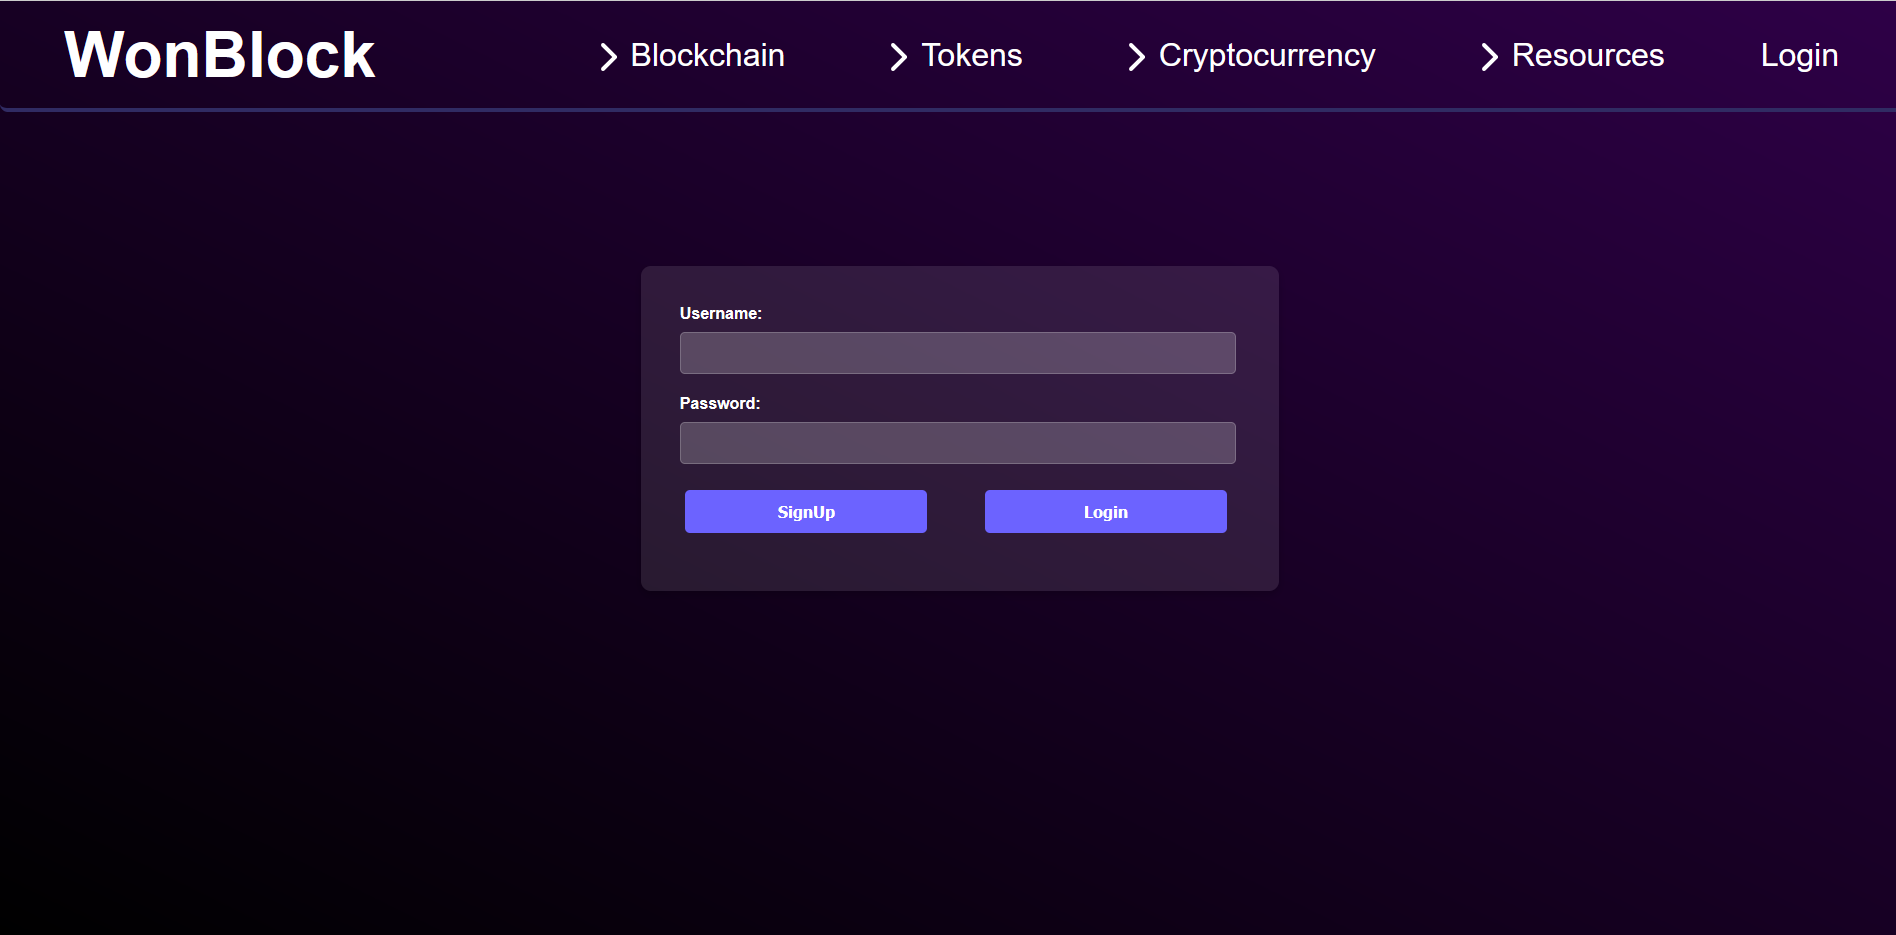
\includegraphics[width=0.8\linewidth]{./instrukcja/Login.png}
    \caption{Logowanie}
    \label{fig:Logowanie}
\end{figure}
Jeżeli użytkownik nie ma konta, należy kliknąć w przycisk \texttt{Sign up}, aby się zarejestrować.

\subsection{Strona główna}
Po zalogowaniu, użytkownik zostanie przeniesiony na główną stronę:
\begin{figure}[htb]
    \centering
    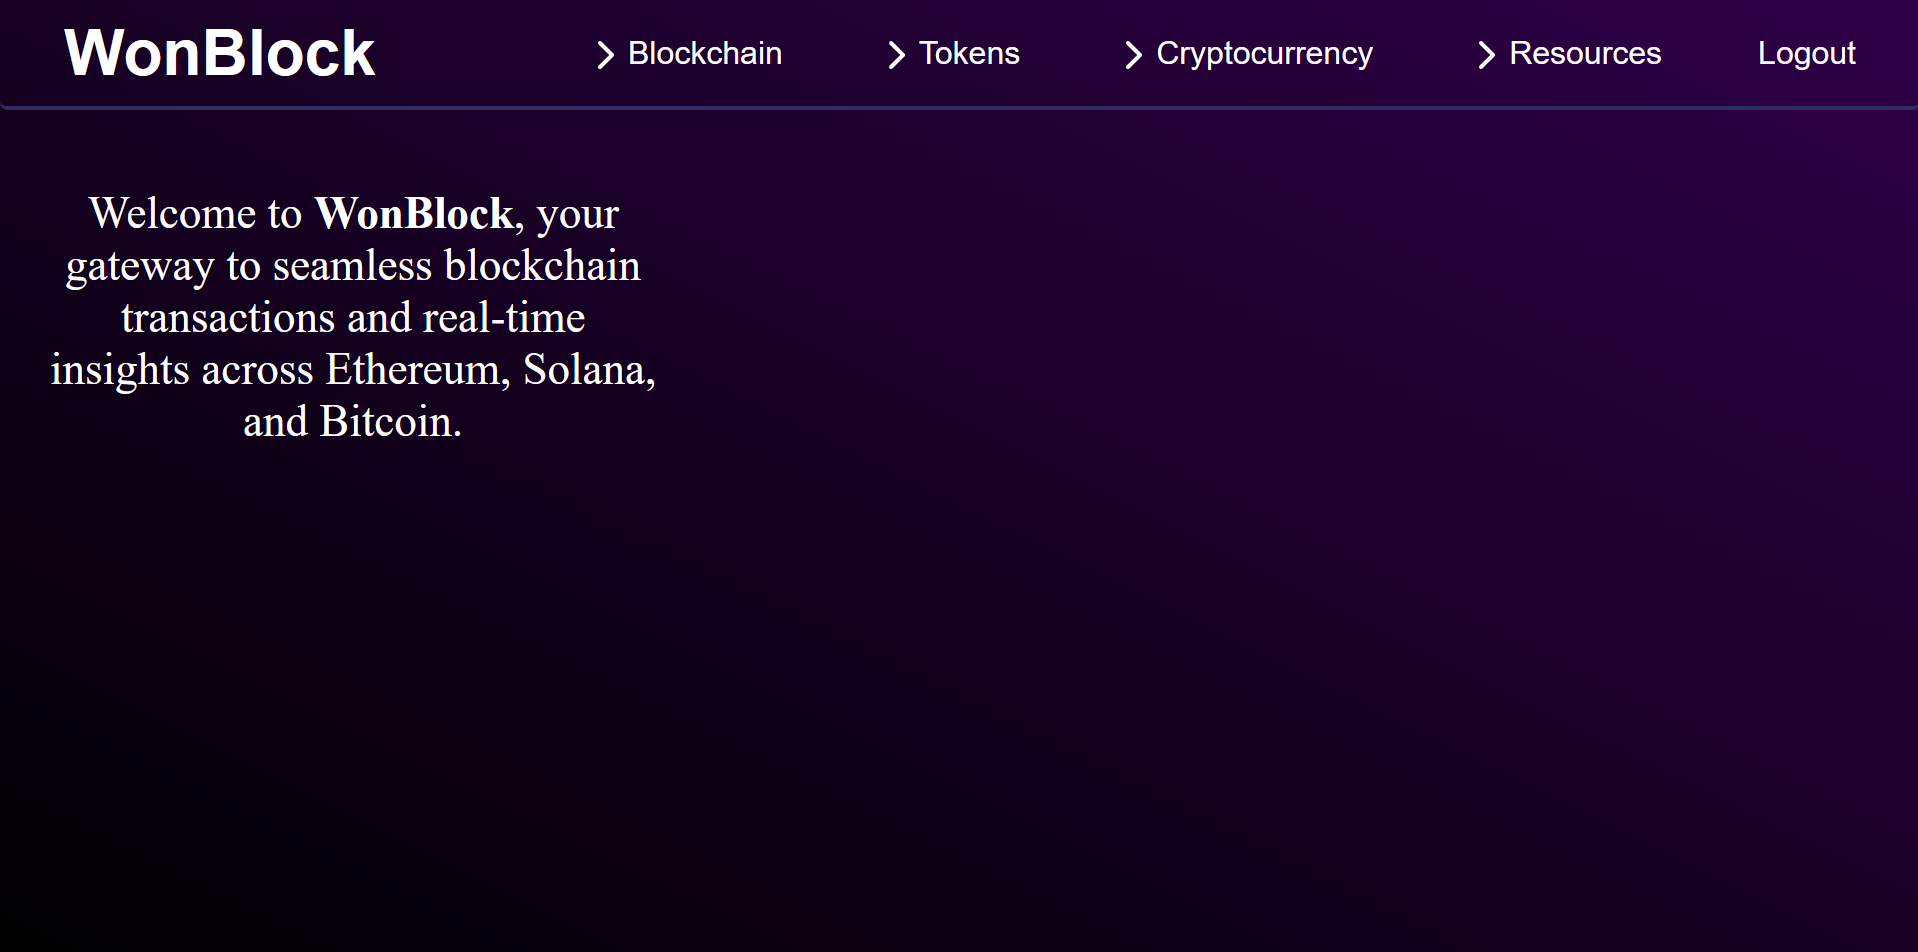
\includegraphics[width=0.8\linewidth]{./instrukcja/mainpage.png}
    \caption{Strona główna}
    \label{fig:Strona główna}
\end{figure}

Na górze każdej strony będzie pasek z opcjami:
\begin{enumerate}
    \item Blockchain
    \item Tokens
    \item Cryptocurrency
    \item Resources
\end{enumerate}
\subsection{Blockchain}
Zakładka blockchain ma możliwość:
\begin{enumerate}
    \item Accounts
    \item View Blocks
    \item Transactions
\end{enumerate}
\subsubsection{Konto}
Aby wyszukować konto należy wpisać adres oraz wybrać blockchain z którego pochodzi dany adres.
\begin{figure}[htb]
    \centering
    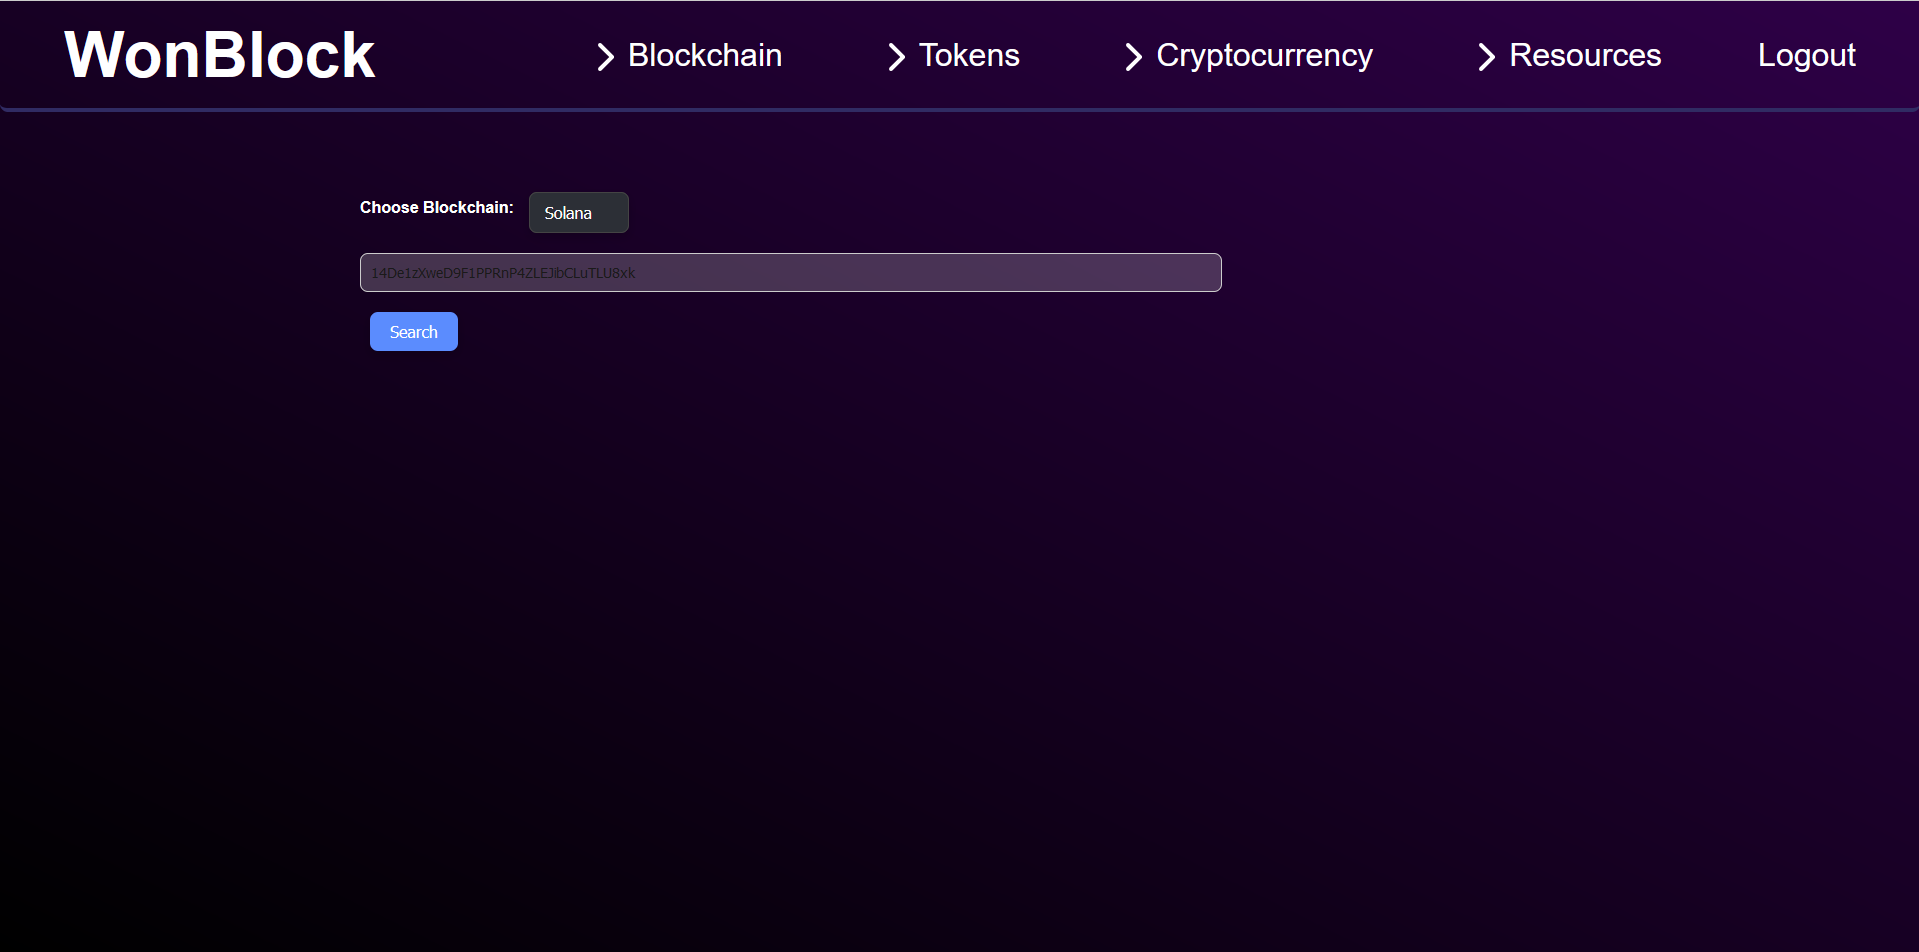
\includegraphics[width=0.8\linewidth]{./instrukcja/Check_account.png}
    \caption{Znajdź konto}
    \label{fig:Znajdź konto}
\end{figure}

Strona automatycznie przeniesie użytkownika na nową stronę z danymi konta:
\begin{figure}[htb]
    \centering
    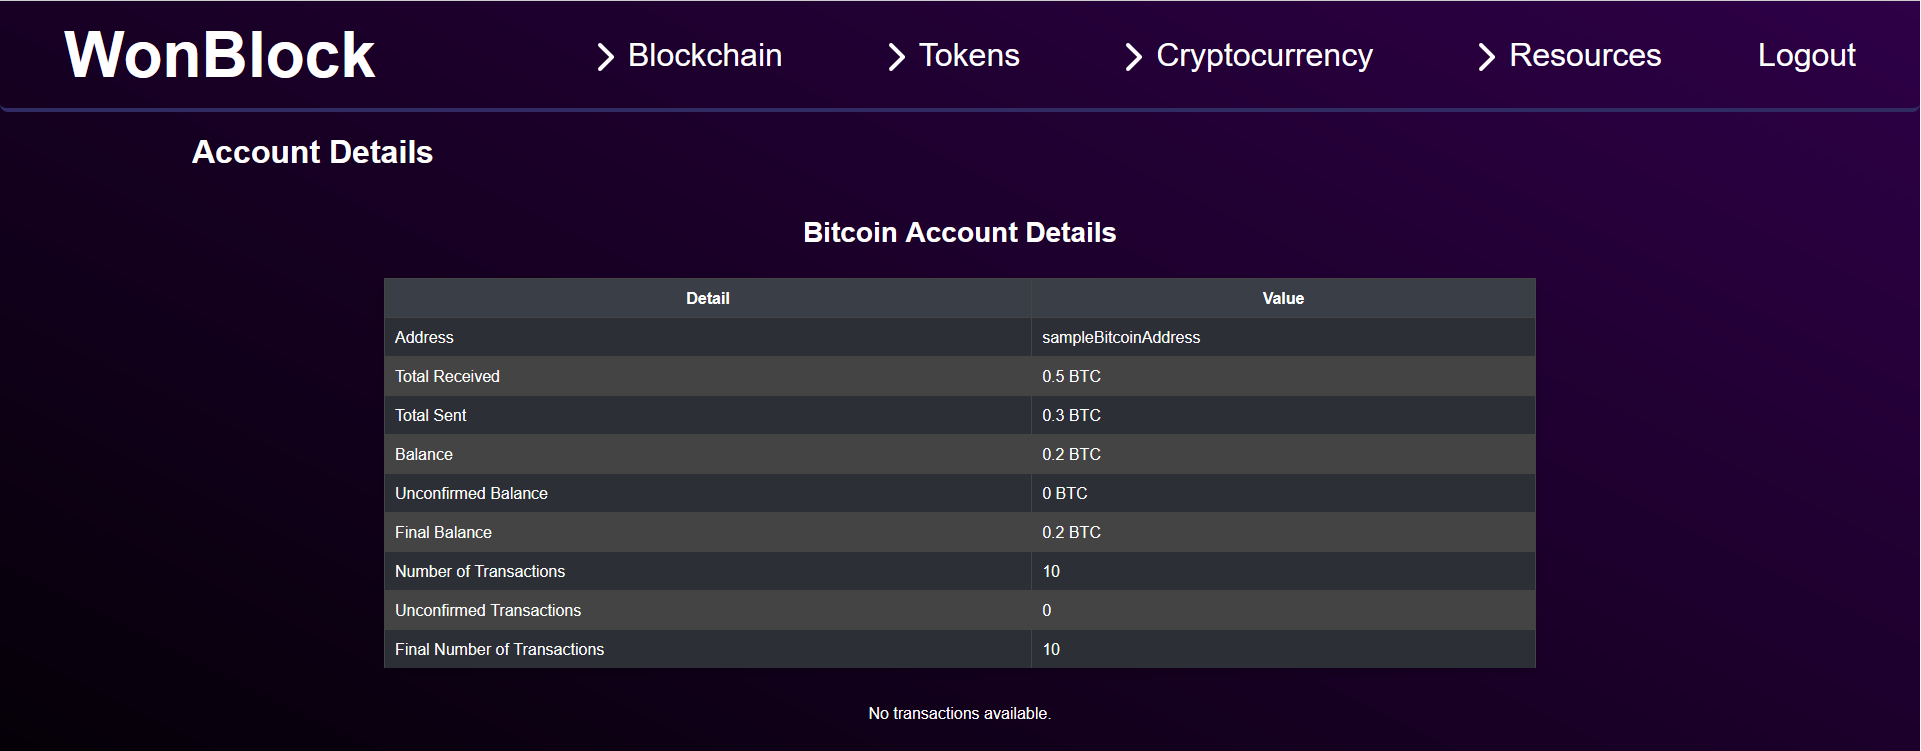
\includegraphics[width=0.8\linewidth]{./instrukcja/Account_details.png}
    \caption{Dane konta}
    \label{fig:Dane konta}
\end{figure}

Sprawdzanie bloków oraz transakcji działa analogicznie.

\subsection{Tokens}
Zakładka \texttt{Tokens} ma dwie opcje:
\begin{enumerate}
    \item Collection
    \item General NFT statistics
\end{enumerate}
\subsubsection{Kolekcje}
Jeśli użytkownik wybierze, opcję Collection, to zostanie przeniesiony na stronę z listami kolekcji:
\begin{figure}[htb]
    \centering
    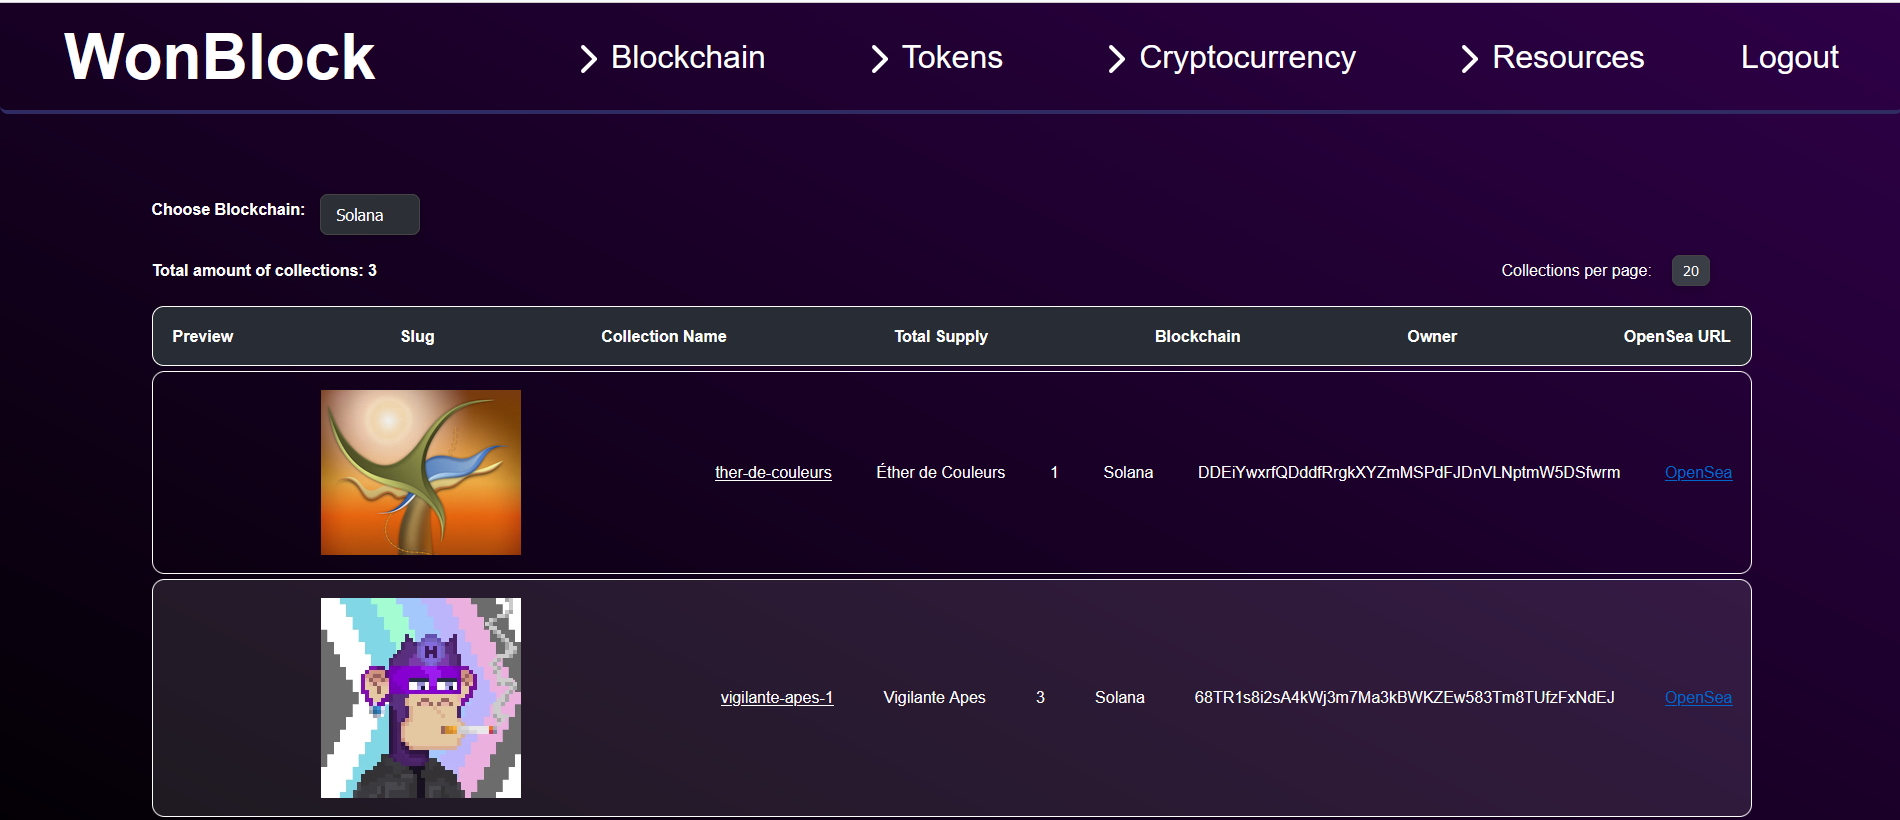
\includegraphics[width=0.8\linewidth]{./instrukcja/Collections.png}
    \caption{Collections}
    \label{fig:Collections}
\end{figure}
\subsubsection{Statystyka}
Drugą opcją jest \texttt{General NFT statistics} po wybraniu, której użytkownik zostanie przeniesiony na stronę:
\begin{figure}[htb]
    \centering
    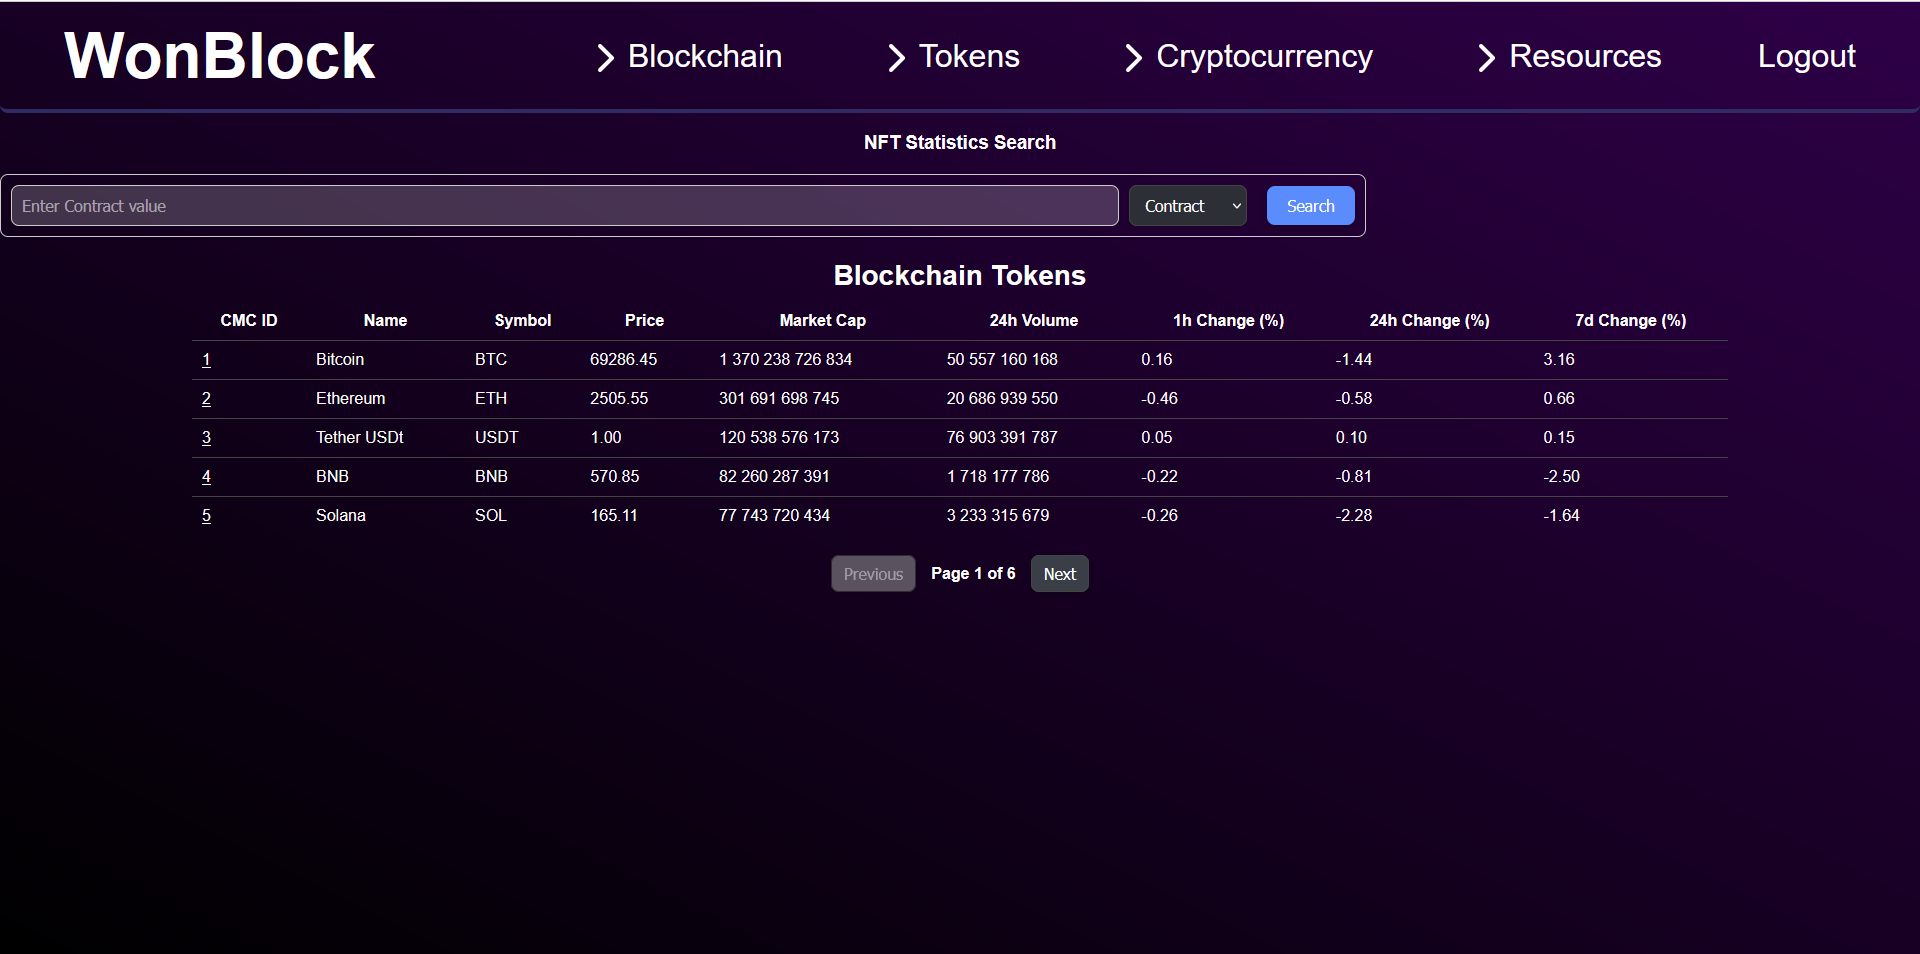
\includegraphics[width=0.8\linewidth]{./instrukcja/Tokens.png}
    \caption{Tokeny}
    \label{fig:Tokeny}
\end{figure}
Na tej stronie użytkownik może szukać tokenów po:
\begin{enumerate}
    \item Kontrakt
    \item Identyfikator
		\item Nazwa
		\item Kolekcja
\end{enumerate}

\subsection{Cryptocurrency}
Następną opcją jest \texttt{Cryptocurrency}, w której użytkownik może wybrać jedną z opcji:
\begin{enumerate}
    \item Ranking
    \item Categories
    \item Global market
    \item Historical data
    \item Gainers \& Losers
\end{enumerate}

\subsubsection{Ranking}
Opcja \texttt{Ranking} Ranking pokaże listę tokenów:
\begin{figure}[htb]
    \centering
    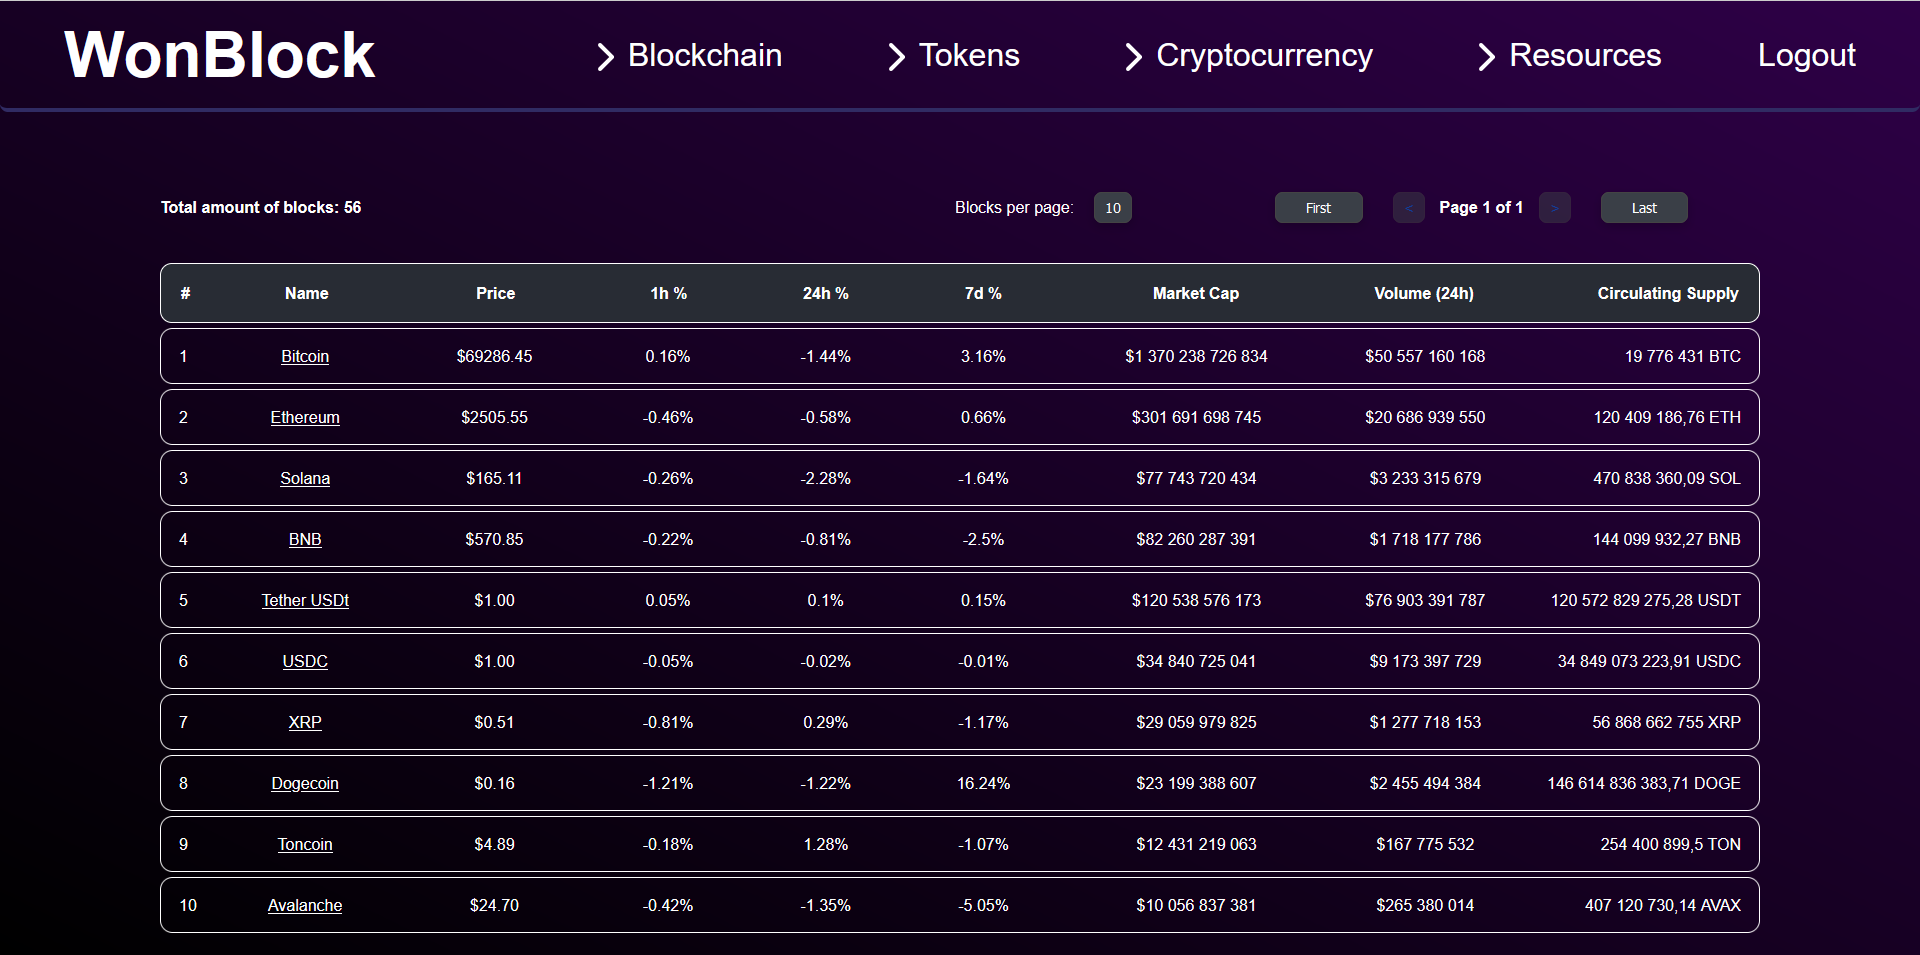
\includegraphics[width=0.8\linewidth]{./instrukcja/Ranking.png}
    \caption{Ranking}
    \label{fig:Ranking}
\end{figure}
\subsubsection{Kategorie}
Opcja \texttt{Categories} pozwala na zobaczenie listy kategorii
\subsubsection{Rynek światowy}
Opcja \texttt{Global market} oraz \texttt{Gainers and Losers} pokazuje wykresy na temat globalnych rynków oraz na statystykę \texttt{Gainers and Losers} odpowiednio.
\subsubsection{Dane historyczne}
Opcja \texttt{Historical Data} pokaże kalendarz, z którego można wybrać dowolną datę sprzed dwóch lat, aby zobaczyć stan rankingu na dany dzień
\begin{figure}[htb]
    \centering
    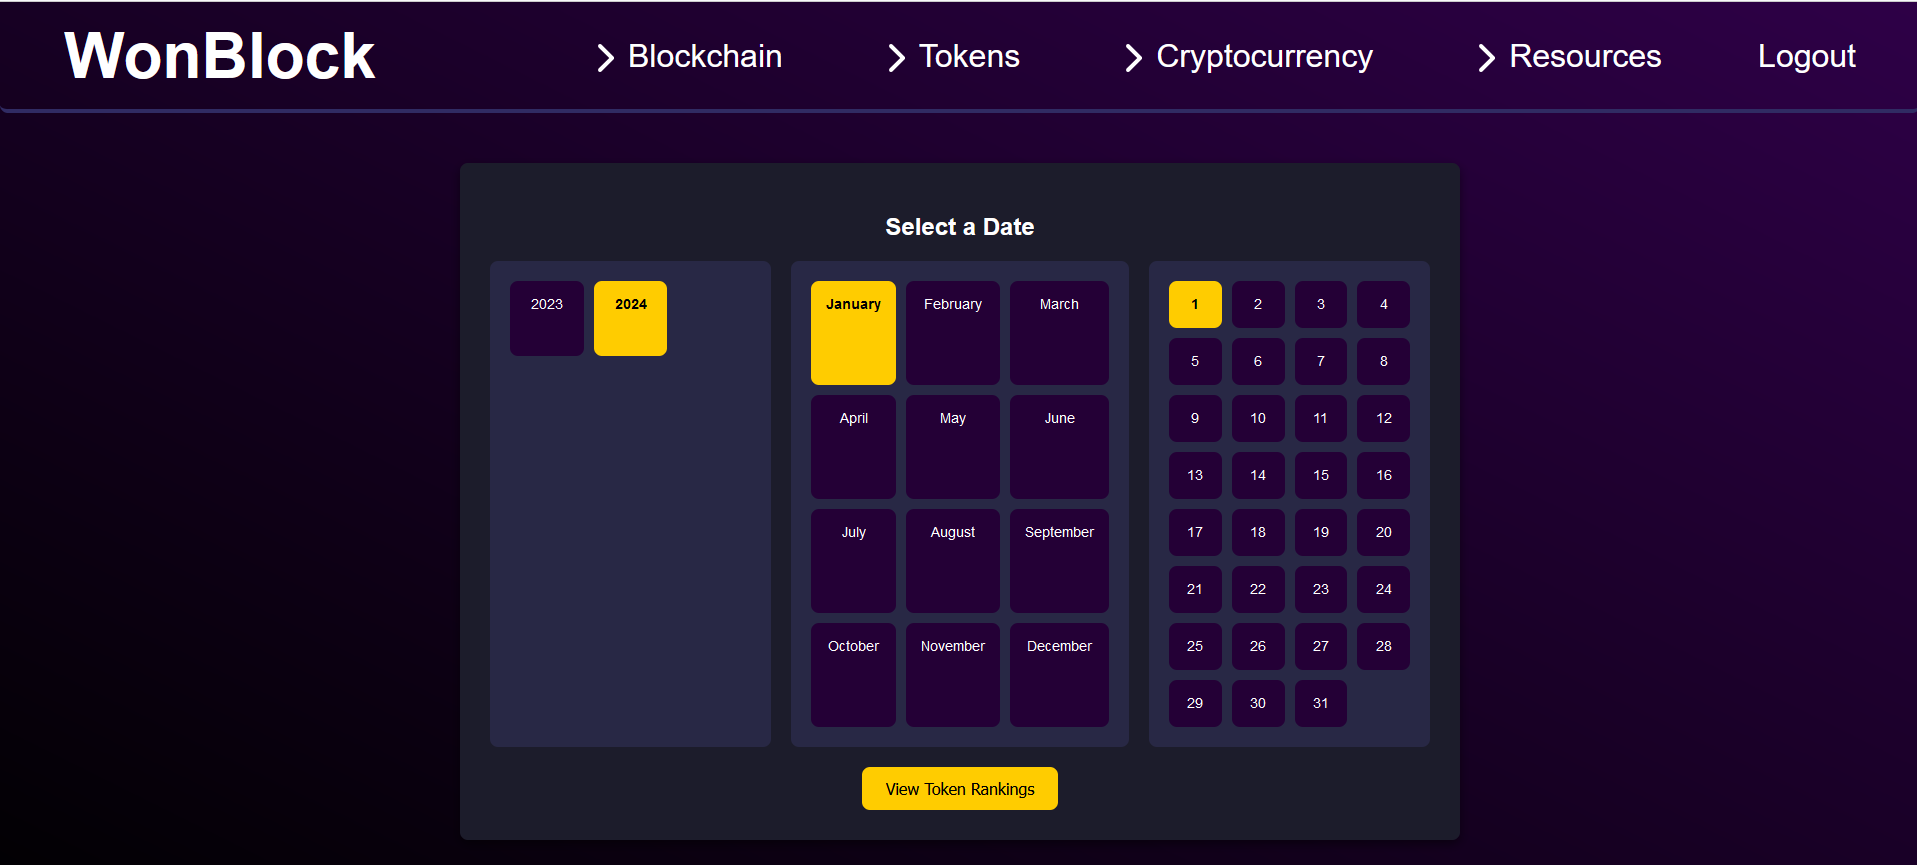
\includegraphics[width=0.8\linewidth]{./instrukcja/HistoricalData.png}
    \caption{Dane historyczne}
    \label{fig:Dane historyczne}
\end{figure}


\subsection{Resources}
Opcja \texttt{Resources} pozwala użytkownikowi na:
\begin{enumerate}
    \item Converter
    \item Directory
    \item News
    \item Simulate Transaction
    \item Predict Prices
\end{enumerate}
\subsubsection{Konwerter} 
Opcja konwerter pozwala na przekonwertowanie walut i kryptowalut:
\begin{figure}[htb]
    \centering
    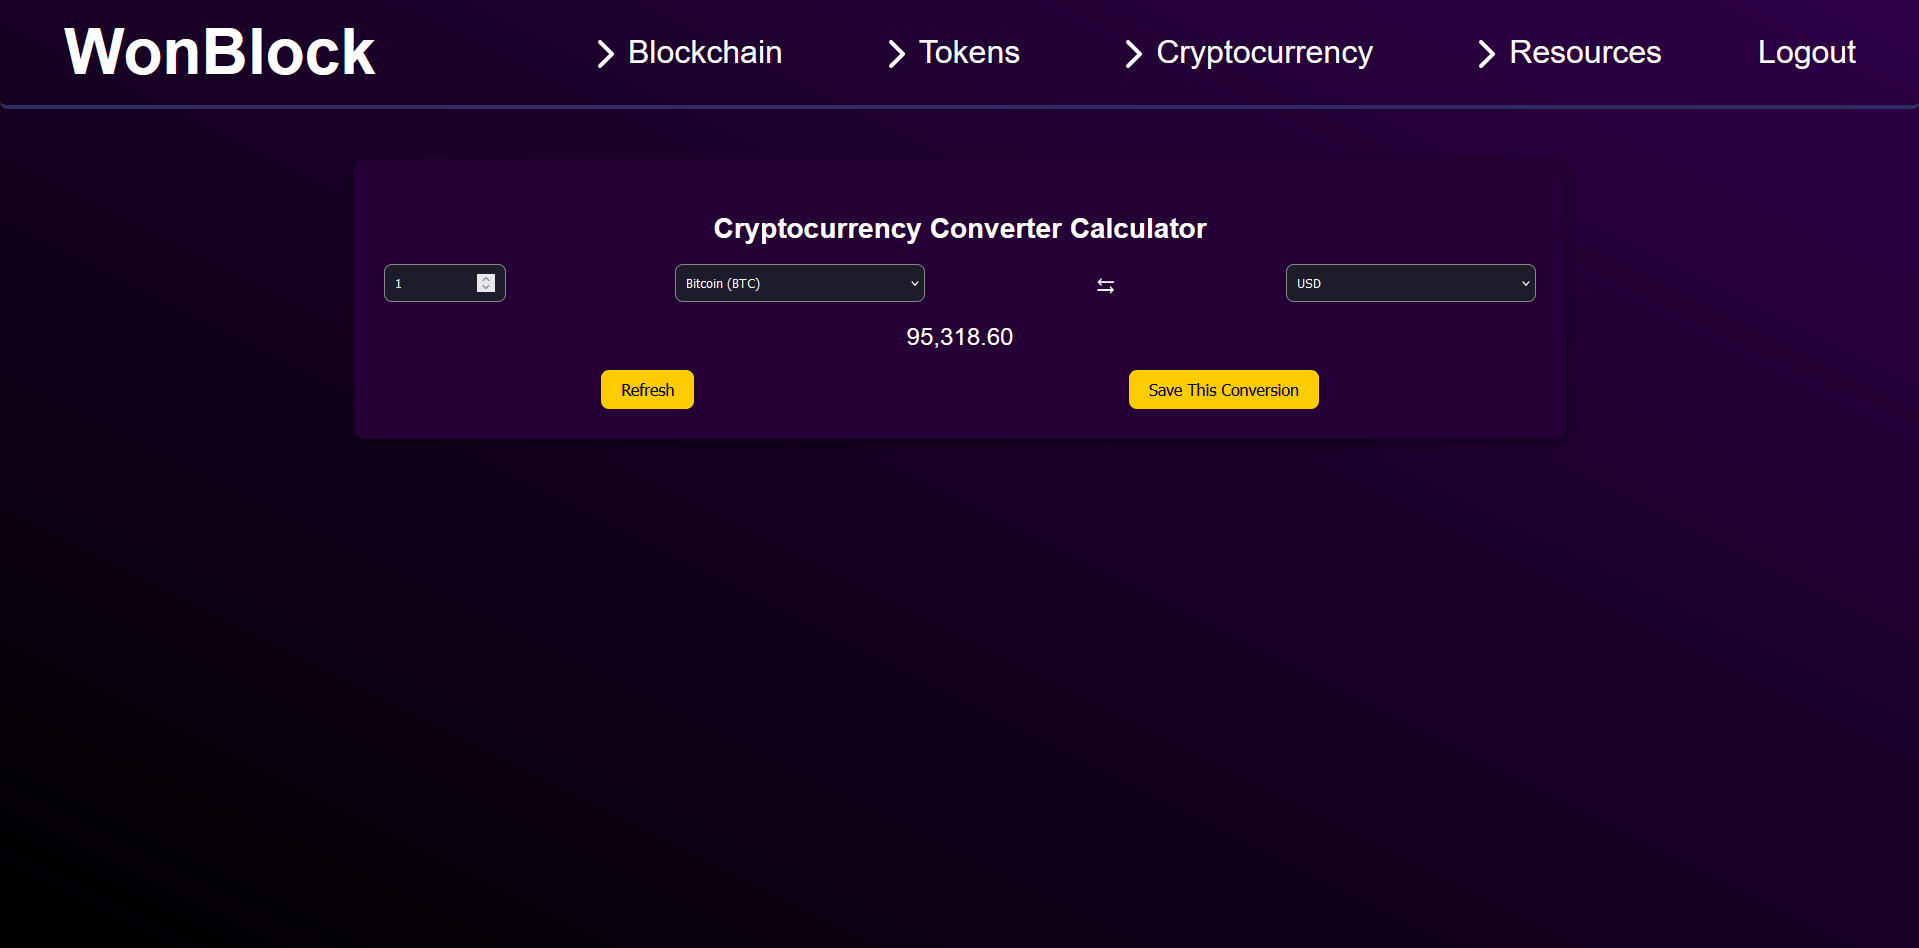
\includegraphics[width=0.8\linewidth]{./instrukcja/Converter.png}
    \caption{Konwerter}
    \label{fig:Konwerter}
\end{figure}

\subsubsection{Nauka}
Opcja \texttt{Directory} zawiera różne źródła, z których użytkownik może się uczyć na temat technologii blockchain.
\subsubsection{Wiadomości}
Opcja \texttt{News} zawiera najnowsze informacje ze świata na temat różnych blockchainów.
\subsubsection{Symulacja transakcji}
Opcja \texttt{Simulate Transaction} pozwala użytkowniki na wpisanie tekstu i zasymulowanie transakcji:

\begin{figure}[htb]
    \centering
    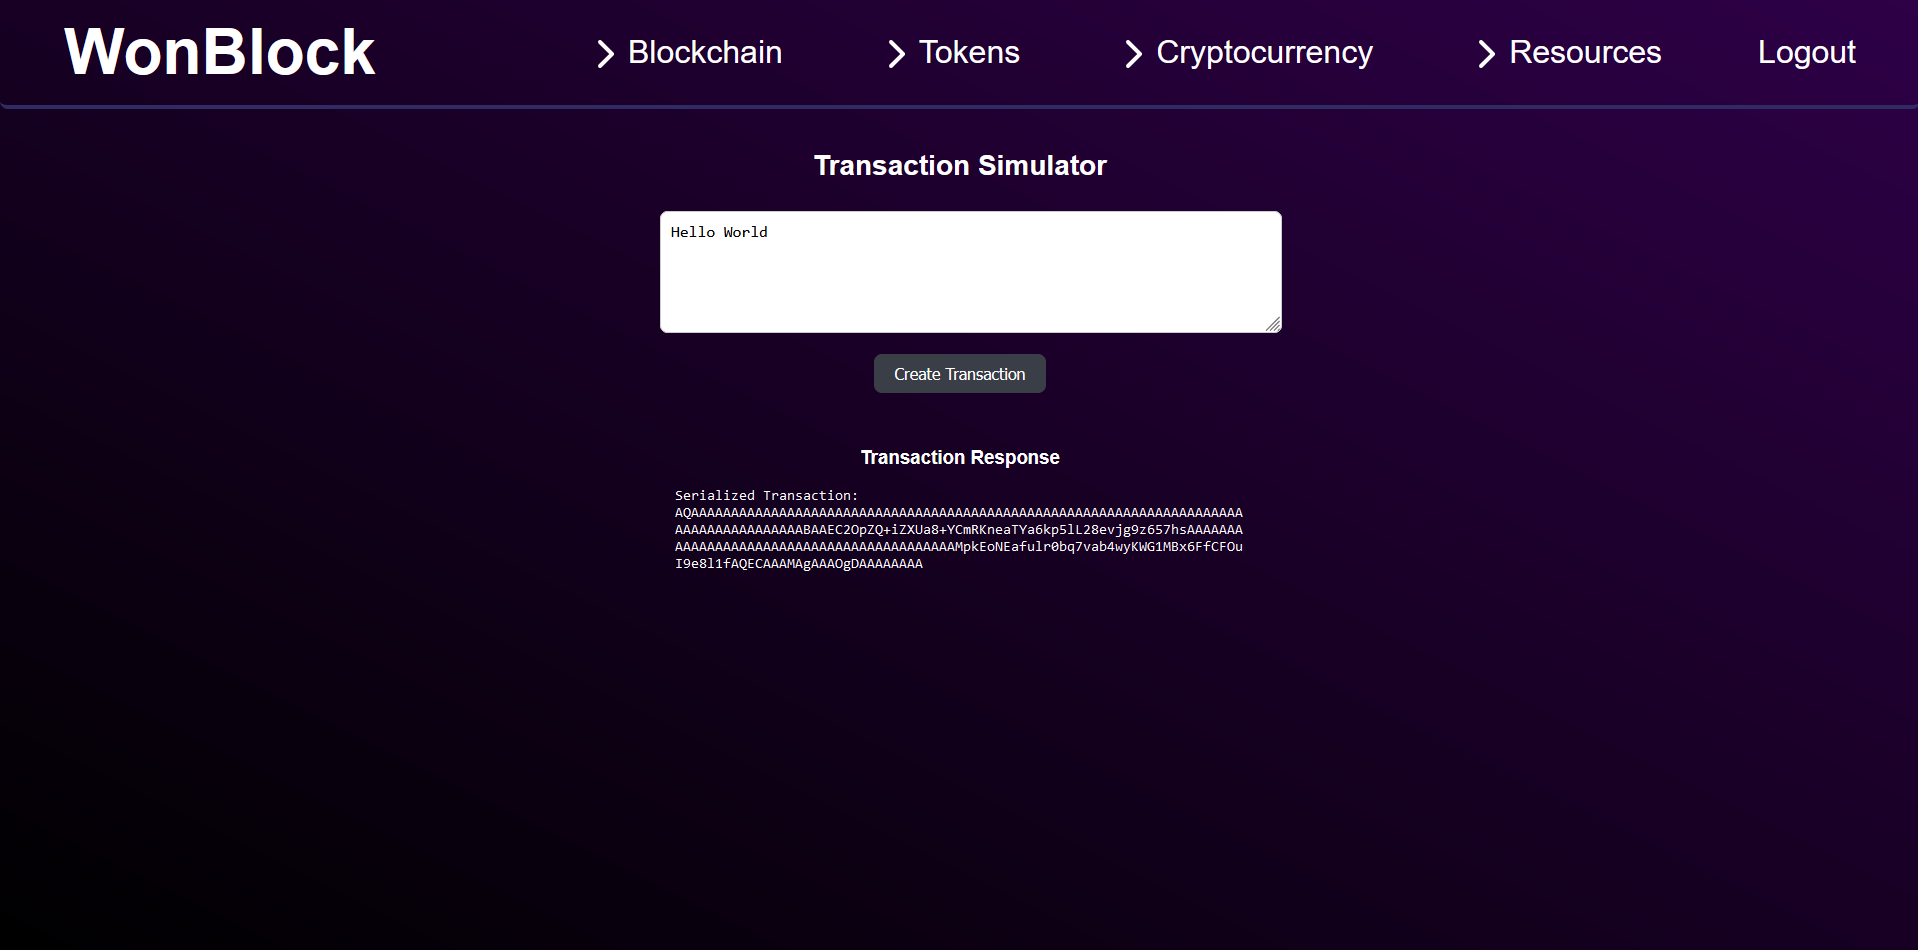
\includegraphics[width=0.8\linewidth]{./instrukcja/SimulateTransaction.png}
    \caption{Symulowanie transakcji}
    \label{fig:Symulowanie transakcji}
\end{figure}

\subsubsection{Przewidywanie cen}
Opcja \texttt{Predict prices} pozwala użytkowniki na poznanie przewidywanych wartości dla kryptowalut Bitcoin, Ether oraz Sol:
\begin{figure}[htb]
    \centering
    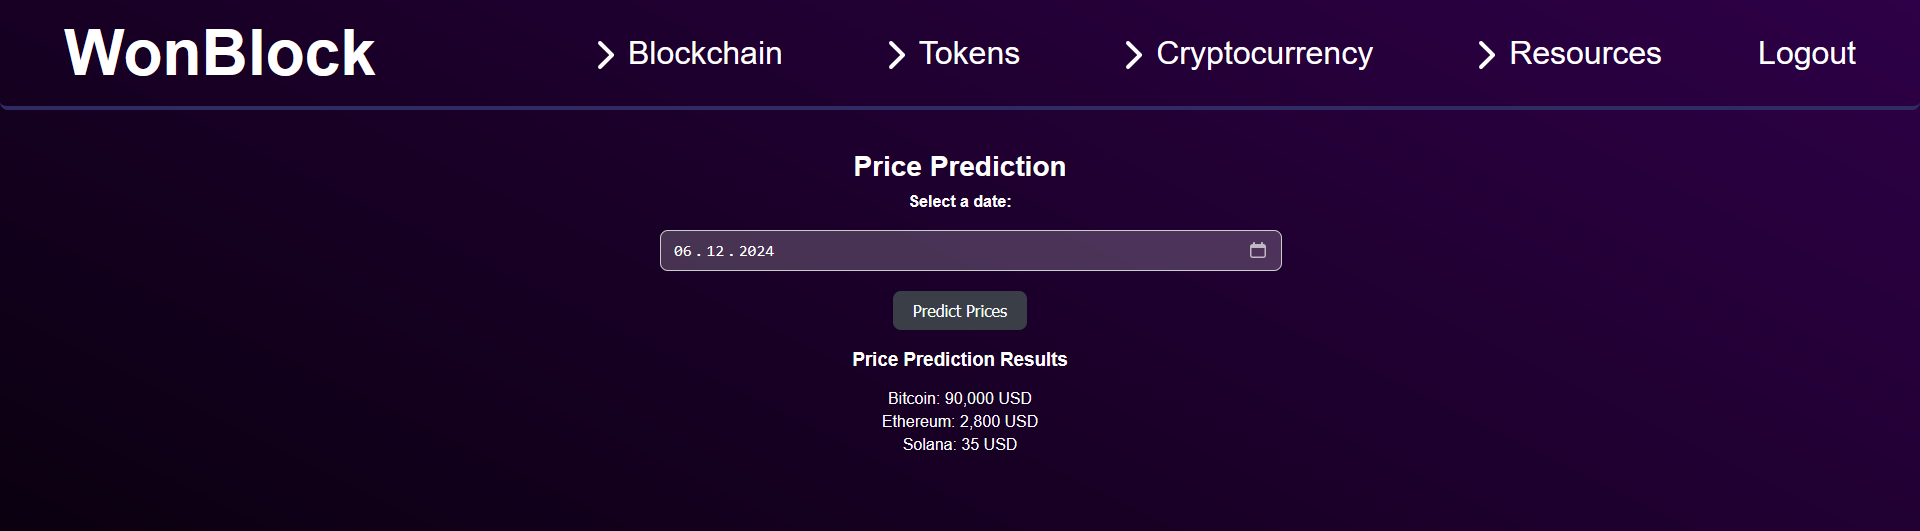
\includegraphics[width=0.8\linewidth]{./instrukcja/PredictPrices.png}
    \caption{Przewidywanie cen}
    \label{fig:Przewidywanie cen}
\end{figure}